\documentclass[11pt]{article}
\usepackage{amsmath,textcomp,amssymb,geometry,graphicx,enumerate}

\def\Name{Vijay Hans}  % Your name
\def\SID{3041285081}  % Your student ID number
\def\Prelab{4} % Number of Prelab
\def\Session{Spring 2026}
\def\Cls{PHYS 5BL}
\title{\Cls--Spring 2026 --- Prelab \Prelab \ Response}
\author{\Name, SID \SID}
\markboth{\Cls -- \Session\  Prelab \Prelab \ \Name}{\Cls -- \Session\ Prelab \Prelab\ \Name}
\pagestyle{myheadings}
\date{\today}

\newenvironment{qparts}{\begin{enumerate}[{(}a{)}]}{\end{enumerate}}
\def\endproofmark{$\Box$}
\newenvironment{proof}{\par{\bf Proof}:}{\endproofmark\smallskip}

\textheight=9in
\textwidth=6.5in
\topmargin=-.75in
\oddsidemargin=0.25in
\evensidemargin=0.25in
\setlength{\parindent}{0pt}
\begin{document}
\maketitle

\begin{enumerate}
    \item Image Below: \\ 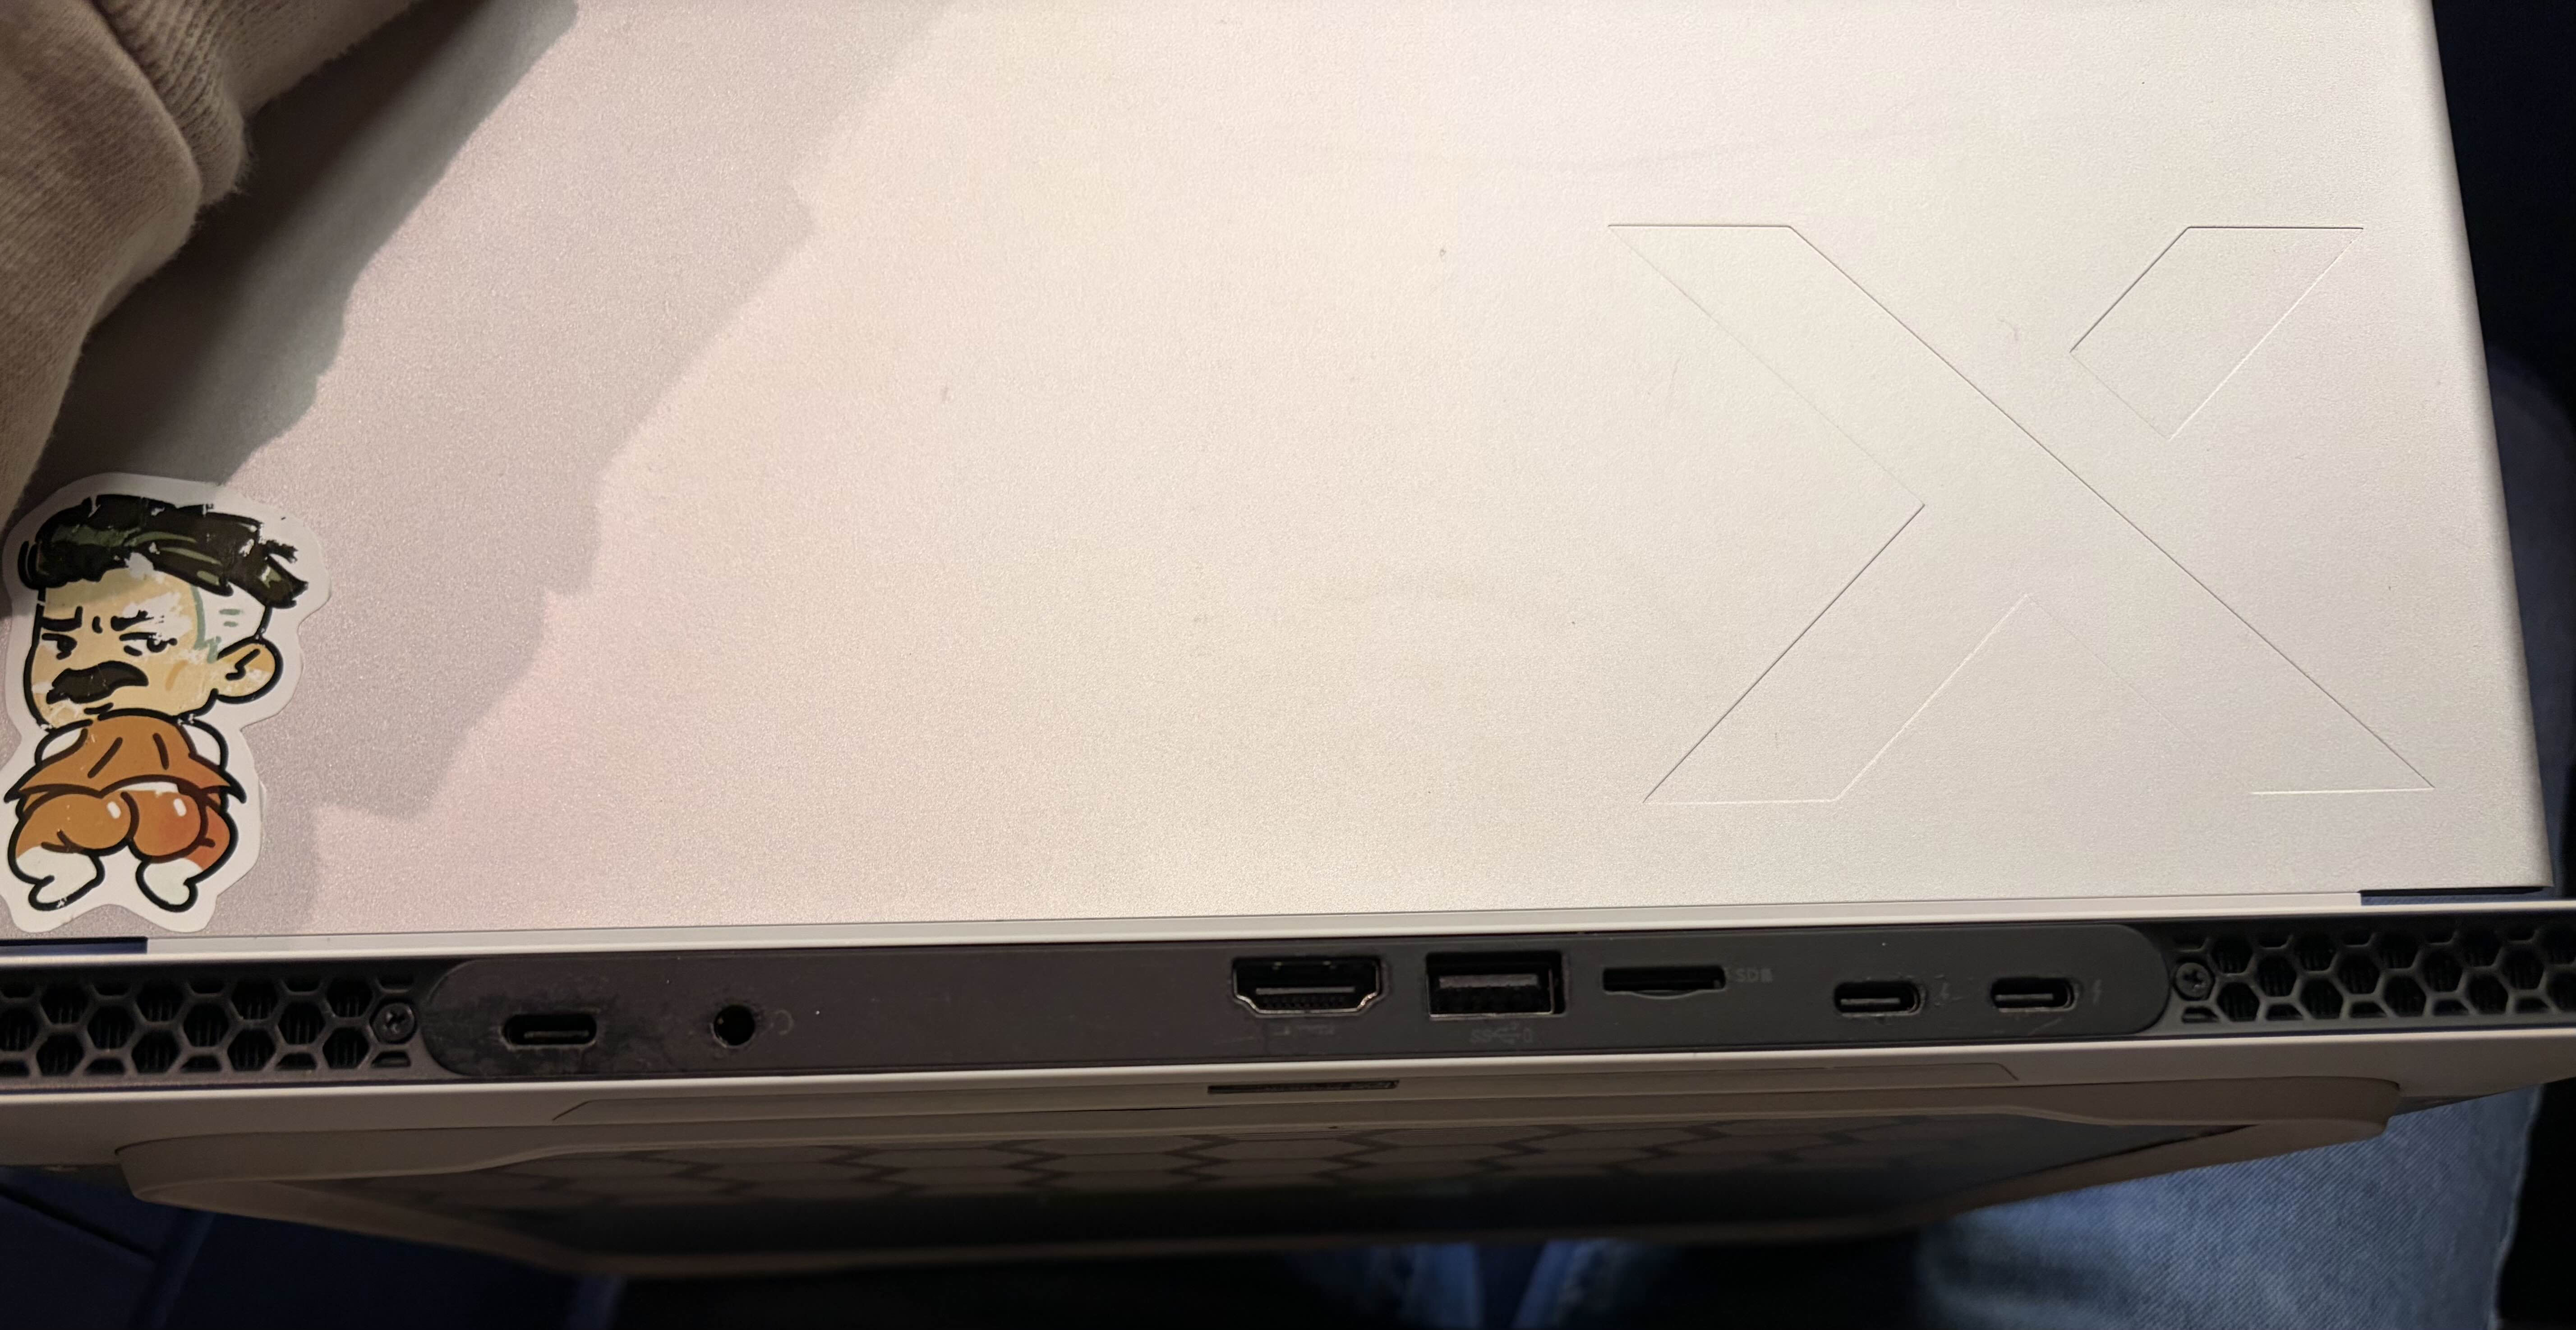
\includegraphics[scale=0.08]{IMG_0428.jpg}
    \item \begin{enumerate}
              \item $P(\text{Double Red} | \text{Red}) = \frac{P(\text{Red} | \text{Double Red}) \cdot P(\text{Double Red})}{P(\text{Red})} = \frac{1 \cdot 1/3}{1/2} = \frac{2}{3}$
              \item You need to verify that all cards with even numbers have blue faces on the other side (so flip over 8) and you that all cards with non-blue faces have non-even numbers (so flip over red).
          \end{enumerate}
\end{enumerate}

\end{document}